\chapter{INTRODUCTION} % Main chapter title
\label{ChapterIntroduction} % For referencing the chapter elsewhere, use \ref{ChapterIntroduction} 

Figure \ref{f1} shows the .. 

\begin{figure}[h]
\begin{center}
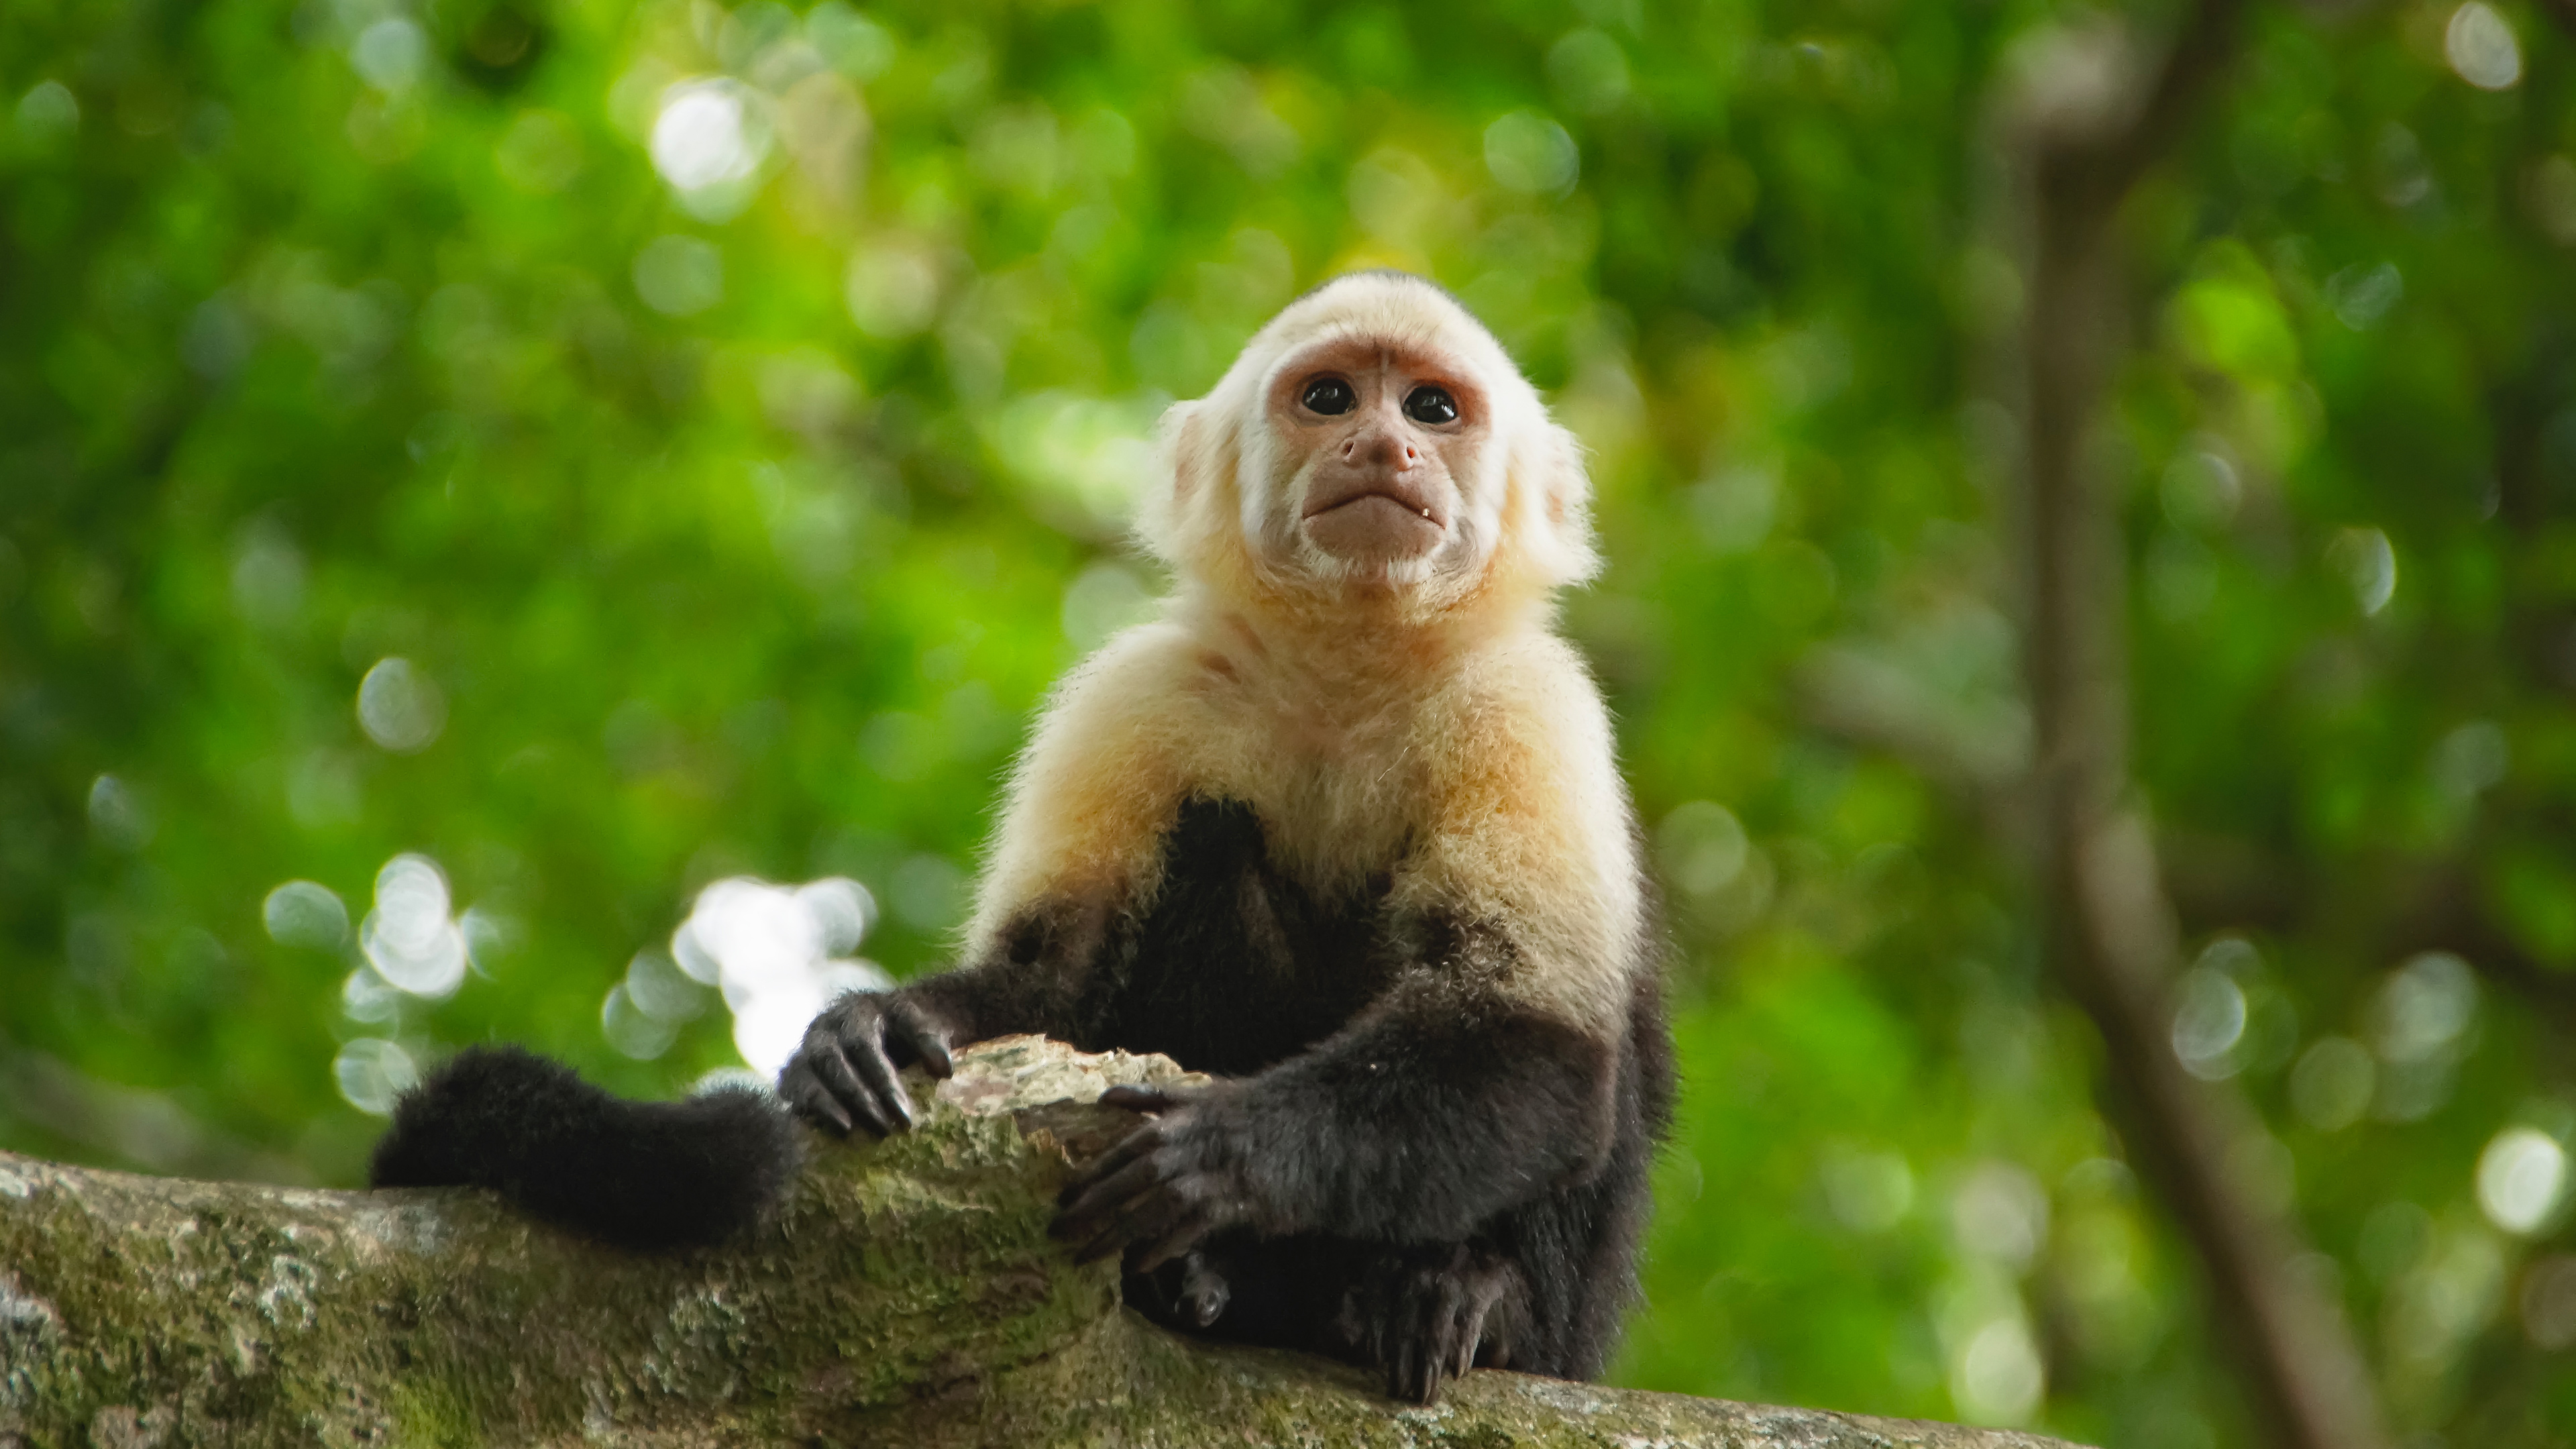
\includegraphics[width=14cm,height=12cm]{Figures/f1.JPG}
\caption[center]{Figure 1}
\label{f1}      
\end{center}
\end{figure}


The report shall not have more than five chapters \cite{lecun2015deep}. The title or heading of these chapters are also fixed except for the Chapter named ‘Actual work’. Students have the flexibility to choose the title for this chapter and its sub chapters. 
\\
The chapter shall also have the following four mandatory sub-chapters:  
	\[F=ma
\]

\begin{itemize}
	\item bfkjgnn
	\item hgjhgj
	\item jgjhbjb
\end{itemize}

\section{Problem Identification}
Under this the reason for choosing the particular problem or title for the project shall be explained along with the thought process that was involved in doing so.
\subsection{Subsection}
This is a subsection.

\begin{table}
\centering
\caption{Sample Table}
\label{t1}
\begin{tabular}{|p{4cm}|p{8cm}|}
\hline
\textbf{Framework } & \textbf{Application } \\
\hline
Research and Ethical Scoping &  privacy, consent, and data bias \\
\hline
Ethical Data Acquisition  & Dataset is anonymized \\
\hline
\end{tabular}
\end{table}

\section{Problem Formulation}
The identified problem shall be formulated in a systematic manner and provide clarity on the problem statement and objectives

	
\section{Problem Statement \& Objectives}
List of project objectives along with the problem statement shall be provided in this section.

\section{Limitations}
This is an academic research based project and has its own limitations with respect to time and other constraints. Also, there might be other limitations of the project work depicted in the reported that may not be obvious from the title. It is very important to mention those limitations and avoid any misconceptions in the minds of the readers and/or evaluators.
